

%%%%%%%%%%%%%%%%%%%%%%%%%%%%%%%%%%%%%%%%%%%%%%%%%%%%%%%
\subsection{Overview of Pion TPC Candidate ID}\label{sec:TPCCandidateSelect}
%%%%%%%%%%%%%%%%%%%%%%%%%%%%%%%%%%%%%%%%%%%%%%%%%%%%%%%
Wherever possible, data and Monte Carlo are treated identically for the analysis specific cuts. The selection criteria were developed for this analysis to identify events in which the measured $\pi, \mu, e$ candidate track from the beamline could be matched to activity within the LArTPC. Selections are made to allow disambiguating the activity in the TPC and matching this to the beamline track as well as attempting to reject activity which comes from electromagnetic showers (e.g. electrons and photons) in the beamline.

\begin{itemize}
\item{\textbf{Require the presence of a track in the upstream portion of the TPC}}\\

To select events which can be well matched to the reconstructed WC-track, we require at least one of the TPC reconstructed tracks to have a spacepoint within the first 2 cm in z coordinate, as shown in Fig.\ref{fig:UsFilter0}. An event is rejected if none of the reconstructed tracks have a space point with $0 < z < 2$ cm. The choice of 2~cm distance was arrived at from MC studies outlined in \href{https://lartpc-docdb.fnal.gov:441/cgi-bin/ShowDocument?docid=1766}{docDB-1766} , \href{https://lartpc-docdb.fnal.gov:441/cgi-bin/ShowDocument?docid=1778}{docDB-1778}, \href{https://lartpc-docdb.fnal.gov:441/cgi-bin/ShowDocument?docid=1784}{docDB-1784}

\item{\textbf{Track Multiplicity Requirement}}\\
To reduce both the number of events with high pile-up as well as to reject events which have an electromagnetic shower developing early in the upstream portion of the TPC, we filter events based on the number of tracks present in the region from 0~cm<$z$<14~cm. If more than three tracks are found in this region, the event is removed. The region 0~cm<$z$<14~cm and the requirements of less than four tracks was chosen by comparing pion MC to electron/photon MC as well as looking at a preliminary sample of data (as outlined in \href{https://lartpc-docdb.fnal.gov:441/cgi-bin/ShowDocument?docid=1766}{docDB-1766} , \href{https://lartpc-docdb.fnal.gov:441/cgi-bin/ShowDocument?docid=1778}{docDB-1778}, \href{https://lartpc-docdb.fnal.gov:441/cgi-bin/ShowDocument?docid=1784}{docDB-1784})

\item{\textbf{Shower Rejection}}\\

Hand-scanning a sample of data from Run-I it was found that after applying the selection criteria previously mentioned, there remained a significant sample of residual electromagnetic showers aligned with beam (see Figure \ref{fig:stillShow}). 

\begin{figure}[h!]
\centering
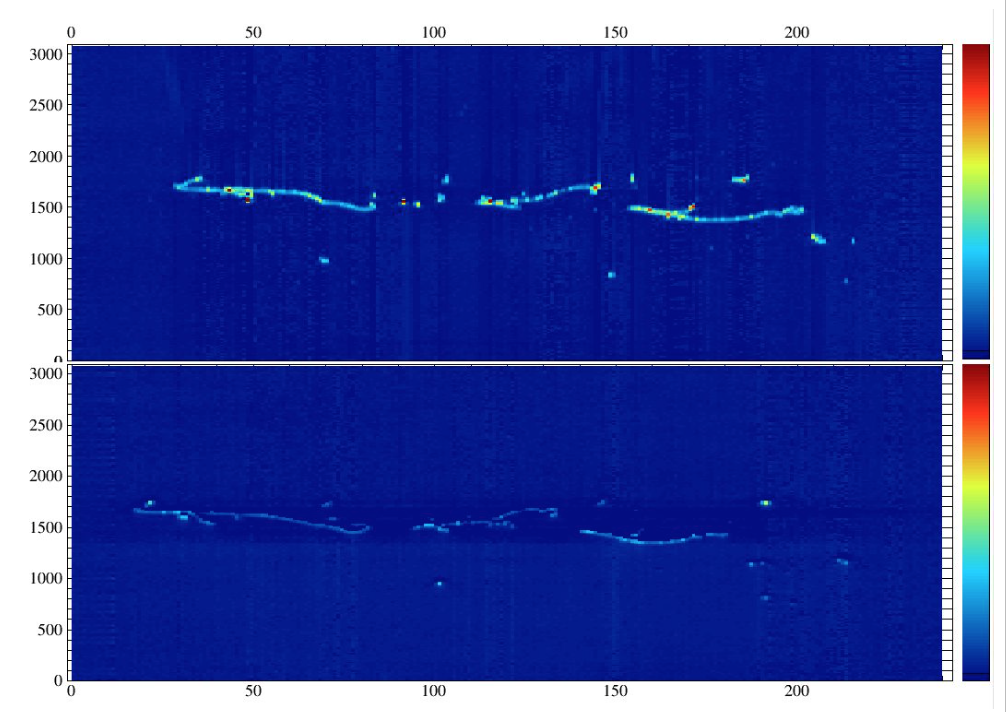
\includegraphics[scale=0.45]{./images/showerEvent.png}
\caption{Example of a "shower-like" event that passes all the previous selection cuts.}
\label{fig:stillShow}
\end{figure}

To eliminate events like this we utilize a simple ``track-based'' filter which, as shown from MC studies, removes a large number of electromagnetic events while still keeping pion events. 

This filter evaluates how many tracks in the TPC are reconstructed for the event and the length for each of these tracks. We then count how many of those tracks would be classified as "short tracks" where ``short'' is any track with length less than 5 cm. Events with more than two ``short'' tracks are removed from consideration. Figure \ref{fig:showrej} shows a graphical representation of this shower based event filter.

\begin{figure}[h!]
\centering
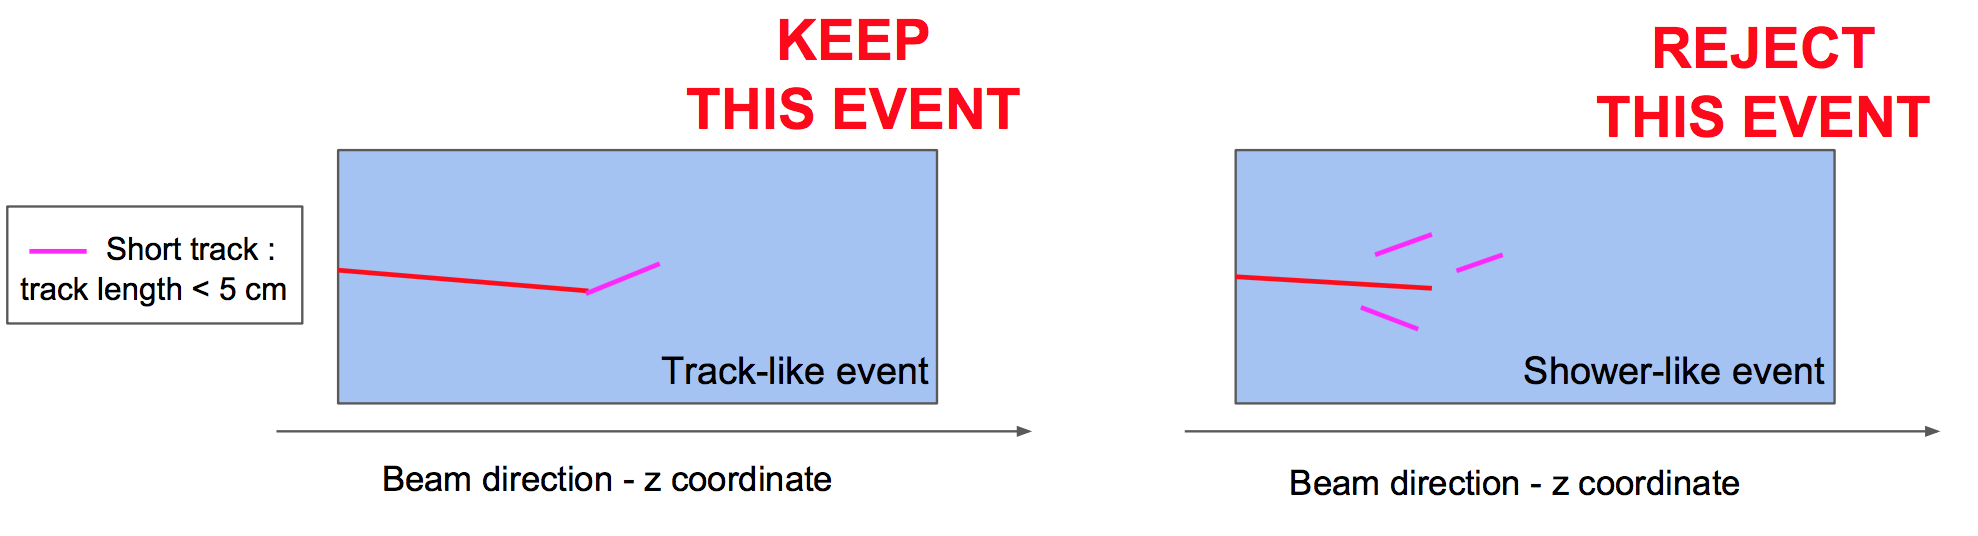
\includegraphics[scale=0.45]{./images/ShowerRejection.png}
\caption{Representation of the Residual Showers Rejection cut.}
\label{fig:showrej}
\end{figure}

The number of ``short'' tracks and the length of the tracks has been chosen utilizing a preliminary scan of the open box data sample and comparing the values to the single particle Monte Carlo attempting to maximize our signal compared to the background.

\item{\textbf{WC to TPC Track Match}}\\

We attempt to uniquely match one WC-Track to one and only one reconstructed TPC track. This match is done to the upstream most point of the TPC track by matching in the $X$ and $Y$ coordinate of the extrapolated WC-Track to the upstream most point of the reconstructed TPC Track as well as matching the incoming track angle to the reconstructed TPC track angle.

We define $\Delta$X as the difference between the $x$ position of the most upstream point of the TPC track and the $x$ position of the WC track as projected to the TPC front face. $\Delta$Y is defined analogously. $\Delta\alpha$ is the angle between the incident WC Track and the TPC track in the plane that contains them. If a Wire Chamber Track to TPC match is found with a  -4~cm~$< \Delta X<$ 6~cm, -5~cm $ < \Delta Y< $~5~cm, and $\alpha < $ 10$^o$ then we consider this a ``well matched'' track. We require each event to have one and only one well matched WC-Track/TPC Track pair.

\begin{figure}[h!]
\centering
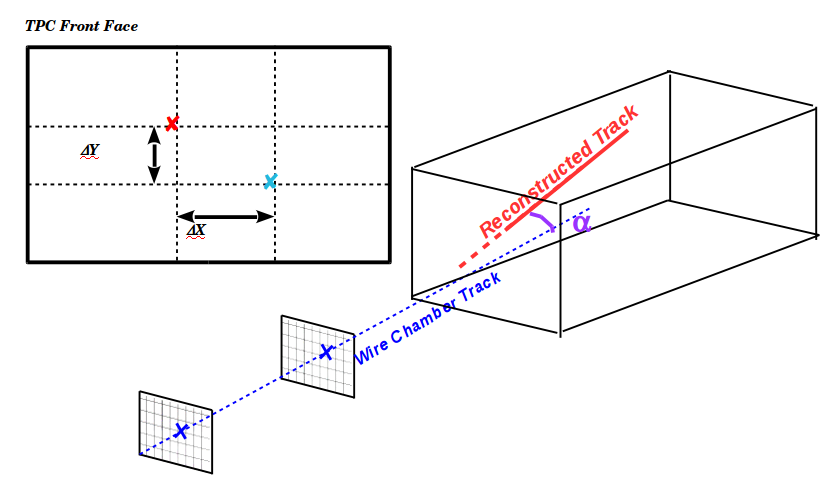
\includegraphics[scale=0.35]{./images/WCTPCMatchSchematic.png}
\caption{Schematic which shows the matching between Wire Chamber tracks and TPC tracks (top) as well as MC particles and TPC tracks.}
\label{fig:WCTrackMatching}
\end{figure}

In the Monte Carlo, there is no reconstructed WC-Track, so instead a projected track from the point of generation is made simulate the WC-Track. The reconstructed MC-track is then matched to this projected point at the front face of the TPC. While this method does not capture the efficiency associated with the wire chamber track algorithm itself, it does allow for a matching based on the data topology and momentum.

\end{itemize}

Having now developed the method by which we select the pion candidate track and have this track uniquely matched to a wire chamber track, we can proceed with analyzing this to establish the cross-section. In order to do this, it is necessary to lay out the general technique used in this analysis.
